\tikzstyle{orbit1}=[rectangle,draw=blue!50,fill=blue!20]
\tikzstyle{orbit2}=[rectangle,draw=green!50,fill=green!20]
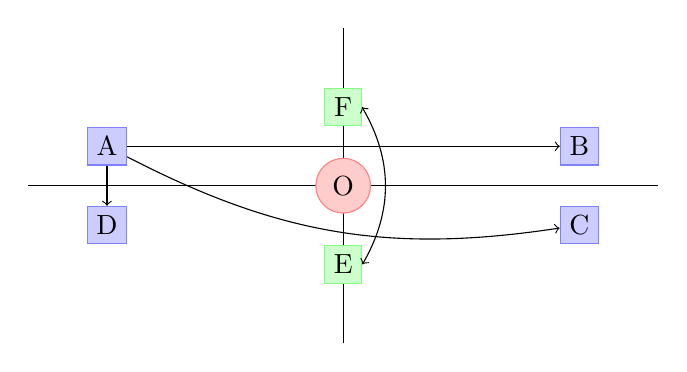
\begin{tikzpicture}
	\draw (-4,0) -- (4,0);
	\draw (0,-2) -- (0,2);

	\node (O) at (0,0) [circle, draw=red!50,fill=red!20] {O};


		\node (A) at (-3.0,0.5) [orbit1] {A};
		\node (B) at (3.0,0.5) [orbit1] {B};
		\node (C) at (3.0,-0.5) [orbit1] {C};
		\node (D) at (-3.0,-0.5) [orbit1] {D};

		\node (E) at (0,-1) [orbit2] {E};
		\node (F) at (0,1)  [orbit2] {F};

	\draw [->] (A) to (B);
	\draw [->] (A) to [bend right=18] (C);
	\draw [->] (A) to (D);

	\draw [<->] (E.east) to [bend right=30] (F.east);


\end{tikzpicture}
